\subsection{Intro}

\begin{theorem}(Division Algoritm)
    Suppose \(a\),\(b\in\Z\) \s s.t. \s \(b>0\).
    Then there are  unique \(q\),\(r \in\Z\) \s s.t. \s \(a=bq+r\) and \(0\leq r < b\)
\end{theorem}
\begin{proof}
    Let \(a\), \(b\in\Z\) s.t. \(b>0\). Consider \(A = \{a-bx | x\in\Z\} \cap\N\)\\
    By the Well Ordering Principle since A has all non-negative terms it has a minimum lets call this \(r\) and call the associated \(x\in\Z\), \(q\).\\
    Thus, \(r=a-bq \implies a=bq+r\).\\
    For contradiction, assume \(r\geq b\).\\
    \(\implies r=b+m\) s.t. \(m\geq0\)\\
    \(\implies b+m=a-bq \implies m=a-b(q+1)\in A \implies m < r = \) minimum \(\contr\)
    Thus \(0 \leq r < b\)\\\\
    Fix  \(q_1,q_2,r_1,r_2\in\Z\) s.t. \(a=bq_1+r_1=bq_2+r_2\) and \(0\leq r_1,r_2<b\).\s\s WLOG let \(r_1>=r_2\)\\
    \(\implies bq_1+r_1=bq_2+r_2 \implies r_1-r_2=b(q_2-q_1) \implies r_1-r_2\) is a multiple of \(b\)\\
    Since \(0\leq r_1,r_2<b \implies 0\leq r_1-r_2<b\)\\
    Since \(r_1-r_2\) is strictly less than \(b\) the only multpiple of \(b\) it could be is \(0\) thus \(r_1=r_2\)\\
    \(\implies q_1=q_2\)
\end{proof}

\begin{lemma}(Bezout's Lemma)
    Suppose \(a\),\(b\in\Z\setminus\left\{ 0 \right\}\). Then there are \(x\),\(y\in\Z\) s.t. \(ax+by=\gcd\left( a,b \right)\).
\end{lemma}
\begin{proof}
    Let \(a\),\(b\in\Z\setminus\left\{ 0 \right\}\). Consider \(A= \left\{ax+by \,|\, x,y\in\Z \right\}\cap\N\)\\
    By the Well Ordering Principle since A has all non-negative terms it has a minimum lets call this \(d\) and call the associated \(x,y\in\Z\), \(u\) and \(v\).\\
    By Theorem 0.1.1 \(\exists q,r \in\Z\) s.t. \(a=dq+r\) and \(0\leq r < d\)\\
    Case 1: \(r=0 \implies d\mid a\)\\
    Case 2: \(0 < r < d \implies r=a-dq \implies r=a-(au+bv)q=a(1-uq)+b(-vq)\in A\)\\
    \(\implies r<d=minimum \contr\)\\
    Thus \(d \mid a\) and similarly \(d \mid b\)\\
    Let \(c\in\N\) s.t. \(c\mid a\) and \(c\mid b\)\\
    \(\implies a=cm\) and \(b=cn\) for \(m,n\in\Z\)\\
    \(d=au+bv=c(mu)+c(mv)=c(mu+mv)\implies c \mid d \implies d=\gcd\left( a,b \right)\)
\end{proof}
\newpage
\begin{algorithm}(Euclidean Algoritm)\\
    Find \(\gcd(272,571)\) and \(x,y\in\Z\) s.t. \(272x+571y=\gcd(272,571)\)
    \begin{equation}
        \begin{aligned}
            571 & = 272 \cdot 2 + 27 \\
            & \begin{tikzpicture}[overlay, remember picture]
               \draw [->, thick] (0.8,0.5) -- (-0.3,-0.2);
                \draw [thick] (1.1,0.5) -- (0.5,0.5);
                \end{tikzpicture} \\
        \end{aligned}
    \end{equation}
    \begin{equation}
        \begin{aligned}
            272 & = 27 \cdot 10 + 2 \\
                & \begin{tikzpicture}[overlay, remember picture]
                    \draw [->, thick] (0.75,0.5) -- (-0.2,-0.2);
                    \draw [thick] (0.9,0.5) -- (0.5,0.5);
                    \end{tikzpicture} \\
        \end{aligned}
    \end{equation}
    \begin{equation}
        \begin{aligned}
            27 & = 2 \cdot 13 + 1 \\
        \end{aligned}
    \end{equation}
    Last term before remainder is zero is \(\gcd\)\\
    \(\gcd\left( 272,571 \right)=1\)
    \begin{align*}
        2&=272-27\cdot10 &\text{Use equation (2)}\\
         &=272(21)-571(10)\\
        1&=(571-272\cdot2)-13(272(21)-571) &\text{Use equation (3) with (2)}\\
         &=571(131)+272(-275)
    \end{align*}
\end{algorithm}
